\documentclass[conference]{IEEEtran}
\usepackage{amsmath,amssymb}
\usepackage{graphicx}
\usepackage{booktabs}
\usepackage{multirow}
\usepackage{cite}
\usepackage[hidelinks]{hyperref}
\usepackage{tikz}
\usetikzlibrary{positioning,arrows.meta}
\hyphenation{Eigen-Score}
\newtheorem{proposition}{Proposition}
\newcommand{\sES}{s_{\mathrm{ES}}}
\newcommand{\sLX}{s_{\mathrm{LX}}}
\newcommand{\sTC}{s_{\mathrm{TC}}}

\begin{document}

\title{Training-Free Fusion of Internal, Lexical and Token-Level Evidence for Hallucination Detection in Large Language Models}

\author{\IEEEauthorblockN{Aayaan Ali Khan, Shlok Bhavsar, Prapti Chotaliya}
\IEEEauthorblockA{Indian Institute of Information Technology Vadodara -- International Campus Diu, India}}

\maketitle

\begin{abstract}
Large language models (LLMs) often produce factually incorrect answers in the same fluent and confident style as correct ones. Sampling-based detectors such as EigenScore estimate the reliability of an answer from the spread of the internal states of several sampled responses, but they cannot distinguish a consistently repeated wrong answer from a correct one. In this paper, we study whether the samples that such a detector already draws contain complementary evidence that the internal-state spread does not capture. We consider three label-free signals computed from the same samples, namely the spread of the hidden-state embeddings (EigenScore), the lexical agreement between the sampled answers, and the token-level confidence of the model, and we combine them with a training-free rank fusion (TRI). We further analyse a tie-breaking variant (CTC) whose gain over lexical agreement can be expressed in closed form. Experiments are performed with Llama-2-7B on 1,000 questions each from CoQA, TriviaQA and NQ-Open under a development and held-out protocol, in which all methods and hypotheses were fixed before the held-out data were analysed. On both held-out datasets, TRI improves the AUROC of EigenScore by 2.7 points, which remains significant after Holm correction, and it is the only evaluated method that improves on EigenScore on all three datasets. The improvement requires no additional generations and no labelled data.
\end{abstract}

\begin{IEEEkeywords}
Hallucination detection, large language models, uncertainty estimation, internal states, rank fusion.
\end{IEEEkeywords}

%=====================================================================
\section{Introduction}
Large Language Models (LLMs) are now used in question answering, search and conversational assistants. However, it has been widely observed that LLMs generate factually incorrect content, a phenomenon known as hallucination~\cite{farquhar2024}. Since a hallucinated answer is written in the same tone as a correct one, it is difficult for a user to identify it. Therefore, hallucination detection, i.e., assigning a reliability score to a generated answer without access to the reference answer, has received increasing attention.

Existing detectors draw on three kinds of evidence. Token-level methods estimate uncertainty from the probabilities of the generated tokens, e.g., perplexity or length-normalised entropy~\cite{malinin2021}. Consistency-based methods sample several answers to the same question and measure their agreement in the language space~\cite{lin2023generating,manakul2023} or after semantic clustering~\cite{kuhn2023,farquhar2024}. Internal-state methods operate on the hidden representations of the model~\cite{chen2024inside,sriramanan2024}. Among the latter, the INSIDE framework~\cite{chen2024inside} proposes EigenScore, which measures the semantic divergence of $K$ sampled answers through the eigenvalues of the covariance matrix of their sentence embeddings.

EigenScore relies on a single kind of evidence. When the model repeats the same incorrect answer in all $K$ samples, the embeddings nearly coincide and EigenScore assigns the answer a low hallucination score, although the token probabilities of that answer may still indicate low confidence. In this paper, we investigate whether such complementary evidence, which is already available in the drawn samples, can be combined with EigenScore without training and without additional generations.

The main contributions of this work are as follows:
\begin{itemize}
\item We formulate a training-free rank fusion (TRI) of internal, lexical and token-level evidence computed from the same $K$ samples, and a tie-breaking variant (CTC) whose gain over lexical agreement is derived in closed form.
\item We evaluate both methods with Llama-2-7B on three question-answering benchmarks under a development and held-out protocol, with paired bootstrap confidence intervals and Holm correction for multiple comparisons.
\item We analyse why the fusion helps through correlation, ablation, fixed false-positive-rate and case-study analyses, and we report the EigenScore variants that did not improve detection.
\item We provide an implementation of the complete pipeline that runs on a single 8~GB consumer GPU.
\end{itemize}

The rest of the paper is organised as follows. Section~\ref{sec:background} describes the problem setting and the EigenScore baseline. Section~\ref{sec:method} presents the proposed fusion methods. Section~\ref{sec:experiments} reports the experimental setup, results and analysis. Section~\ref{sec:related} reviews related work, and Section~\ref{sec:conclusion} concludes the paper with limitations and future scope.

%=====================================================================
\section{Background on Hallucination Detection}\label{sec:background}
\textbf{Problem setting.} Let $\mathcal{M}$ be an LLM and $x$ an input question. The model generates an answer $y$, and a hallucination detector computes a score $g(x,y)\in\mathbb{R}$, where a higher value indicates a more likely hallucination. At deployment, an answer is flagged when $g(x,y)>\tau$ for a threshold $\tau$. Since the reference answer is unknown at deployment, $g$ must be computed from the model alone. The quality of $g$ is evaluated by the area under the receiver operating characteristic curve (AUROC), which equals the probability that a randomly chosen hallucinated answer receives a higher score than a randomly chosen correct answer.

\textbf{Sampling-based detection.} Following Chen et al.~\cite{chen2024inside}, $K$ answers $\{y_1,\dots,y_K\}$ are sampled for each question. Three families of scores can be computed from these samples:
\begin{itemize}
\item \emph{Token-level confidence.} The length-normalised entropy (LN-Entropy) averages, over the $K$ samples, the negative log-likelihood of each sample divided by its length~\cite{malinin2021}.
\item \emph{Lexical agreement.} Lexical Similarity is the mean pairwise ROUGE-L~\cite{lin2004rouge} between the $K$ samples~\cite{lin2023generating}; low agreement indicates a likely hallucination.
\item \emph{Internal-state spread.} EigenScore, described below.
\end{itemize}

\textbf{EigenScore.} Let $\mathbf{z}_k\in\mathbb{R}^d$ be the hidden state of the last token of answer $y_k$ at the middle layer of $\mathcal{M}$, and let $Z=[\mathbf{z}_1,\dots,\mathbf{z}_K]\in\mathbb{R}^{d\times K}$. With the centring matrix $J_d=I_d-\frac1d\mathbf{1}_d\mathbf{1}_d^\top$, the covariance matrix of the answers is $\Sigma=Z^\top J_d Z\in\mathbb{R}^{K\times K}$, and EigenScore is defined as
\begin{equation}
\mathrm{ES}(x)=\frac{1}{K}\log\det\left(\Sigma+\alpha I_K\right)=\frac{1}{K}\sum_{i=1}^{K}\log\lambda_i ,
\label{eq:es}
\end{equation}
where $\lambda_1,\dots,\lambda_K$ are the eigenvalues of $\Sigma+\alpha I_K$ and $\alpha=10^{-3}$ is a regularisation term~\cite{chen2024inside}. Up to constants, Eq.~(\ref{eq:es}) is the differential entropy of a Gaussian fitted to the sentence embeddings. Consistent answers produce small eigenvalues and a low score, whereas divergent answers produce a high score.

\textbf{Limitations of EigenScore.} Eq.~(\ref{eq:es}) depends only on the geometry of the $K$ embeddings. Consequently, (i) if all samples are identical, $\Sigma\approx 0$ and EigenScore attains its minimum regardless of whether the shared answer is correct, and (ii) the token probabilities, which the model computes for every generated token at no extra cost, are not used.

%=====================================================================
\section{Method}\label{sec:method}
\subsection{Three Signals from the Same Samples}
For every question, we draw $K=10$ samples and compute the three scores of Section~\ref{sec:background}: EigenScore at layer 16 of 32 ($\sES$), the negative Lexical Similarity ($\sLX$) and LN-Entropy ($\sTC$). Each score is oriented so that a higher value indicates a more likely hallucination, and we refer to them as the internal, lexical and token signals, respectively. The hidden states and token log-probabilities are recorded during sampling, so no further generation is required. Figure~\ref{fig:method} illustrates the overall procedure.

\begin{figure}[t]
\centering
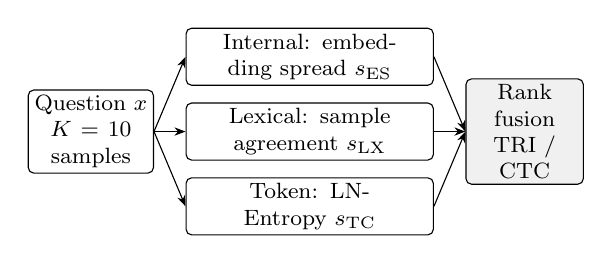
\begin{tikzpicture}[font=\footnotesize, >={Stealth[length=4pt]},
  box/.style={draw, rounded corners=2pt, align=center, minimum height=0.7cm, inner sep=2pt}]
\node[box, text width=1.45cm] (q) {Question $x$\\$K=10$\\samples};
\node[box, right=0.4cm of q, text width=3.0cm, yshift=0.95cm] (a) {Internal: embedding spread $\sES$};
\node[box, right=0.4cm of q, text width=3.0cm] (b) {Lexical: sample agreement $\sLX$};
\node[box, right=0.4cm of q, text width=3.0cm, yshift=-0.95cm] (c) {Token: LN-Entropy $\sTC$};
\node[box, right=0.4cm of b, text width=1.35cm, fill=black!6] (t) {Rank fusion\\TRI / CTC};
\draw[->] (q.east) -- (a.west); \draw[->] (q.east) -- (b.west); \draw[->] (q.east) -- (c.west);
\draw[->] (a.east) -- (t.west); \draw[->] (b.east) -- (t.west); \draw[->] (c.east) -- (t.west);
\end{tikzpicture}
\caption{Overview of the proposed approach. Three label-free signals are computed from the same $K$ sampled answers and combined by rank fusion. No training and no additional generation are required.}
\label{fig:method}
\end{figure}

\subsection{TRI: Rank Fusion}
The three signals are measured on unrelated scales. Instead of normalising their values, we combine their ranks. For a pool of $N$ questions, let $r(\cdot)$ denote the normalised rank of a score within the pool. The fused score is
\begin{equation}
\mathrm{TRI}(x)=\frac13\Big[r\big(\sES(x)\big)+r\big(\sLX(x)\big)+r\big(\sTC(x)\big)\Big].
\label{eq:tri}
\end{equation}
The weights are equal and no parameter is fitted, so TRI requires no labelled data. At deployment, the rank of a new answer is computed against an unlabelled reference pool of earlier questions, i.e., $r(\cdot)$ is the empirical cumulative distribution function of each signal on that pool.

\subsection{CTC: Consistency, then Confidence}
Lexical agreement is often exactly tied between questions, mostly when all $K$ samples are identical. AUROC counts a tied (hallucinated, correct) pair as one half. CTC orders the questions by $\sLX$ and breaks exact ties by $\sTC$:
\begin{equation}
\mathrm{CTC}(x)=r_{\mathrm{dense}}\big(\sLX(x)\big)+\frac{1}{2N}\Big(r\big(\sTC(x)\big)-\frac12\Big),
\label{eq:ctc}
\end{equation}
where $r_{\mathrm{dense}}$ assigns consecutive integer ranks to the distinct values of $\sLX$.

\begin{proposition}\label{prop:ctc}
Let $\mathcal{P}$ be the set of (hallucinated, correct) pairs, $\mathcal{T}\subseteq\mathcal{P}$ the pairs that are tied under $\sLX$, and $a$ the AUROC of $\sTC$ restricted to $\mathcal{T}$. Then
\begin{equation}
\mathrm{AUROC}(\mathrm{CTC})-\mathrm{AUROC}(\sLX)=\Big(a-\frac12\Big)\frac{|\mathcal{T}|}{|\mathcal{P}|}.
\end{equation}
\end{proposition}
\begin{IEEEproof}
Dense ranks of distinct values differ by at least one, whereas the absolute value of the second term of Eq.~(\ref{eq:ctc}) is below one half. Hence, CTC preserves the order of every untied pair, and these pairs contribute equally to both AUROCs. A tied pair contributes $\frac12$ under $\sLX$, while under CTC it contributes one if $\sTC$ orders it correctly, one half if $\sTC$ is also tied, and zero otherwise. Averaging over $\mathcal{T}$ gives $a$ instead of $\frac12$, and weighting by $|\mathcal{T}|/|\mathcal{P}|$ yields the result.
\end{IEEEproof}

Proposition~\ref{prop:ctc} shows that CTC can only decrease AUROC if token confidence is worse than chance within the tied pairs, and that its gain grows with the fraction of ties. CTC therefore targets the self-consistent case in which all samples agree and token confidence is the only remaining evidence.

%=====================================================================
\section{Experiments}\label{sec:experiments}
\subsection{Experimental Setup}
\textbf{Datasets.} We use three question-answering benchmarks: CoQA~\cite{reddy2019coqa}, a conversational reading-comprehension dataset; TriviaQA~\cite{joshi2017triviaqa} in the closed-book (no context) setting; and NQ-Open~\cite{lee2019latent}, the open-domain version of Natural Questions~\cite{kwiatkowski2019natural}. For each dataset, 1,000 questions are drawn at random from the validation split with a fixed seed. For CoQA, the prompt contains the story and the previous gold question--answer turns; for TriviaQA and NQ-Open, a fixed five-shot prompt is used.

\textbf{Model and sampling.} All experiments use Llama-2-7B~\cite{touvron2023llama} loaded with 4-bit NF4 weights~\cite{dettmers2023qlora} on a single 8~GB laptop GPU (NVIDIA RTX~4060). Following Chen et al.~\cite{chen2024inside}, $K=10$ answers are sampled per question with temperature 0.5, top-$p$ 0.99 and top-$k$ 5, and a greedy answer is decoded for labelling. Generation stops at a newline, with at most 32 new tokens for CoQA and 20 otherwise.

\textbf{Feature extraction.} Hidden states are obtained in a second forward pass that encodes the prompt once and reuses its key--value cache for all $K$ answers. Compared with a full forward pass, the maximum relative difference of the resulting embeddings was $2\times10^{-3}$. The last-token hidden states of all 33 hidden-state layers are stored, which enables the per-layer analysis in Section~\ref{sec:analysis} without regenerating answers.

\textbf{Correctness and metrics.} Following Chen et al.~\cite{chen2024inside}, an answer is labelled as a hallucination when the ROUGE-L F-score between the greedy answer and every reference answer is at most 0.5. The model accuracy under this criterion is 81.4\% on CoQA, 69.9\% on TriviaQA and 26.9\% on NQ-Open. We report AUROC and the true positive rate (TPR) at fixed false positive rates (FPR).

\textbf{Evaluation protocol.} All methods were developed on CoQA only, which serves as the development set. The definitions of TRI and CTC and the hypotheses to be tested were committed to version control before any result on TriviaQA or NQ-Open, the held-out sets, was computed. Differences in AUROC are evaluated with a paired bootstrap over questions with 10,000 resamples. The family of one-sided superiority tests on the held-out sets is corrected with the Holm procedure~\cite{holm1979}, and a hypothesis is regarded as confirmed only if it holds on both held-out datasets.

\textbf{Baselines.} We compare against Perplexity of the greedy answer, LN-Entropy, Lexical Similarity and EigenScore~\cite{chen2024inside}. In addition to TRI and CTC, two further fusions were fixed before the held-out analysis: HYB, the rank average of a multi-layer EigenScore and LN-Entropy, and PMF, which weights the samples by their probability and measures the probability mass that agrees with the greedy answer. They are reported for completeness.

\subsection{Main Results}
Table~\ref{tab:auroc} reports the AUROC of all methods. No single signal is the strongest on every dataset: Lexical Similarity is the best single signal on CoQA and TriviaQA, whereas on NQ-Open, where the model answers only 26.9\% of the questions correctly, all single signals remain between 74.8\% and 76.7\%. TRI achieves 84.6\%, 83.2\% and 79.5\%, respectively. Its mean AUROC (82.4\%) is comparable to that of PMF (82.5\%) and CTC (82.2\%), but TRI is the only method that exceeds EigenScore significantly on all three datasets.

\begin{table}[t]
\centering
\caption{AUROC (\%) on 1,000 questions per dataset with Llama-2-7B. CoQA is the development set; TriviaQA and NQ-Open are held out. The best value in each column is shown in bold.}
\label{tab:auroc}
\footnotesize
\setlength{\tabcolsep}{3.5pt}
\begin{tabular}{@{}llcccc@{}}
\toprule
& Method & CoQA & TriviaQA & NQ-Open & Mean \\
\midrule
\multirow{4}{*}{Baselines} & Perplexity & 74.6 & 79.8 & 74.8 & 76.4 \\
& LN-Entropy & 77.8 & 80.6 & 76.0 & 78.1 \\
& Lexical Similarity & 85.3 & 82.5 & 76.6 & 81.5 \\
& EigenScore~\cite{chen2024inside} & 80.1 & 80.5 & 76.7 & 79.1 \\
\midrule
\multirow{2}{*}{Other fusions} & HYB & 82.0 & 82.0 & 78.3 & 80.8 \\
& PMF & \textbf{87.1} & \textbf{83.7} & 76.6 & \textbf{82.5} \\
\midrule
\multirow{2}{*}{Proposed} & CTC & 85.7 & \textbf{83.7} & 77.1 & 82.2 \\
& TRI & 84.6 & 83.2 & \textbf{79.5} & 82.4 \\
\bottomrule
\end{tabular}
\end{table}

Table~\ref{tab:held} lists the pre-registered tests on the held-out datasets. TRI improves on EigenScore by 2.7 points on both TriviaQA and NQ-Open (Holm-corrected $p<0.001$), and on the development set by 4.5 points (95\% CI $[+2.7,+6.2]$). CTC improves on Lexical Similarity on both held-out sets, in agreement with Proposition~\ref{prop:ctc}, but its improvement over EigenScore is not significant on NQ-Open. HYB and PMF improve on EigenScore on TriviaQA only.

\begin{table*}[t]
\centering
\caption{Pre-registered comparisons on the held-out datasets: difference in AUROC (points) with 95\% paired bootstrap confidence interval and Holm-corrected one-sided $p$-value.}
\label{tab:held}
\small
\setlength{\tabcolsep}{4pt}
\begin{tabular}{@{}lccccc@{}}
\toprule
& \multicolumn{2}{c}{TriviaQA} & \multicolumn{2}{c}{NQ-Open} & \\
\cmidrule(lr){2-3}\cmidrule(lr){4-5}
Comparison & $\Delta$ [95\% CI] & $p_{\mathrm{Holm}}$ & $\Delta$ [95\% CI] & $p_{\mathrm{Holm}}$ & Holds on both \\
\midrule
TRI $>$ EigenScore & $+2.7$ [$+1.7$, $+3.8$] & $<0.001$ & $+2.7$ [$+1.3$, $+4.2$] & $<0.001$ & yes \\
CTC $>$ Lexical Sim. & $+1.2$ [$+0.6$, $+1.8$] & $<0.001$ & $+0.5$ [$+0.2$, $+0.7$] & $<0.001$ & yes \\
CTC $>$ EigenScore & $+3.2$ [$+1.7$, $+4.8$] & $<0.001$ & $+0.3$ [$-1.9$, $+2.6$] & 1.000 & no \\
HYB $>$ EigenScore & $+1.5$ [$+0.3$, $+2.7$] & 0.038 & $+1.5$ [$0.0$, $+3.1$] & 0.124 & no \\
PMF $>$ EigenScore & $+3.2$ [$+1.7$, $+4.7$] & $<0.001$ & $-0.1$ [$-2.5$, $+2.3$] & 1.000 & no \\
PMF $>$ Lexical Sim. & $+1.1$ [$+0.6$, $+1.8$] & $<0.001$ & $0.0$ [$-0.9$, $+1.0$] & 1.000 & no \\
Lexical Sim. $>$ EigenScore & $+2.1$ [$+0.6$, $+3.5$] & 0.018 & $-0.1$ [$-2.4$, $+2.2$] & 1.000 & no \\
\midrule
TRI $\geq$ Lexical Sim. $-$ 1 & $+0.7$ [$-0.4$, $+1.8$] & -- & $+2.9$ [$+1.3$, $+4.5$] & -- & yes \\
\bottomrule
\end{tabular}
\end{table*}

Figure~\ref{fig:roc} shows the ROC curves of TRI and its three input signals. On the held-out datasets, the curve of TRI lies on or above the best single signal over most of the range, and on NQ-Open the separation is largest at false positive rates below 0.2.

\begin{figure*}[t]
\centering
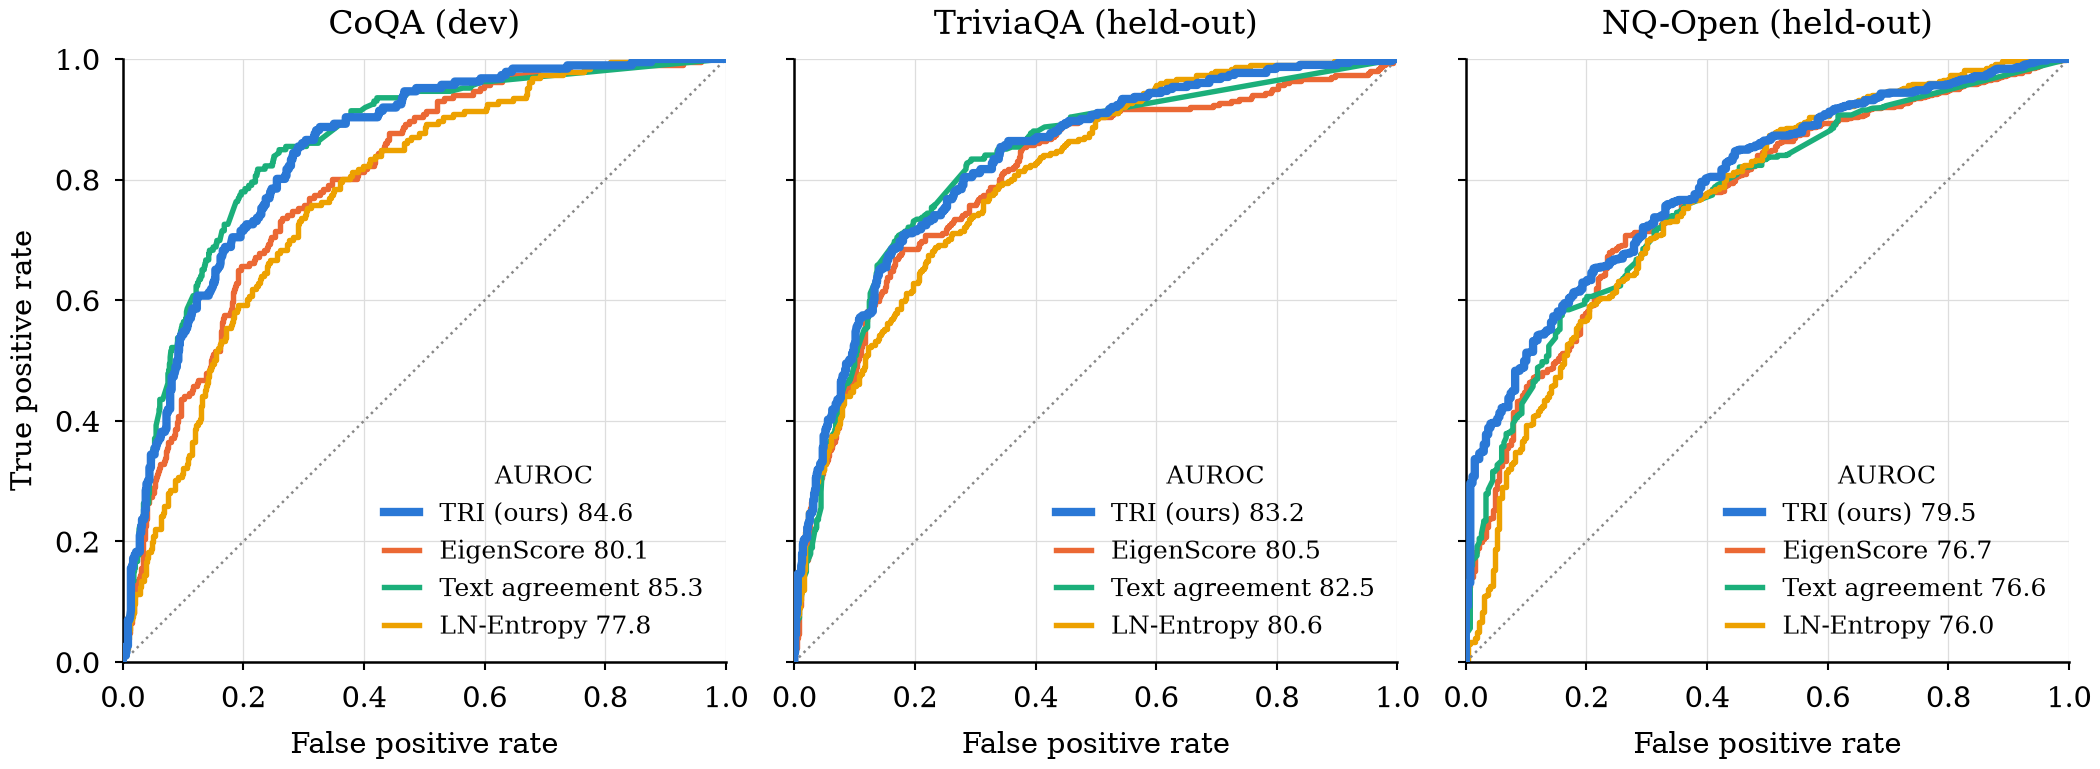
\includegraphics[width=\textwidth]{figures/roc_curves.png}
\caption{ROC curves of TRI and its three input signals on the development set (CoQA) and the two held-out sets. Text agreement denotes Lexical Similarity. The dotted line corresponds to random guessing.}
\label{fig:roc}
\end{figure*}

\textbf{Detection at a fixed false positive rate.} A deployed detector operates at a fixed and usually low false positive rate. Table~\ref{tab:tpr} reports the fraction of hallucinations that are flagged when 5\% or 10\% of the correct answers may be flagged by mistake. On NQ-Open at 5\% FPR, TRI flags 39.7\% of the hallucinations, compared with 28.7\% for EigenScore. On TriviaQA, the corresponding gain is 4.6 points. On CoQA, TRI is close to Lexical Similarity, which is the strongest single signal on that dataset.

\begin{table}[t]
\centering
\caption{True positive rate (\%) at a fixed false positive rate of 5\% and 10\%.}
\label{tab:tpr}
\footnotesize
\setlength{\tabcolsep}{3.5pt}
\begin{tabular}{@{}lcccccc@{}}
\toprule
& \multicolumn{2}{c}{CoQA} & \multicolumn{2}{c}{TriviaQA} & \multicolumn{2}{c}{NQ-Open} \\
\cmidrule(lr){2-3}\cmidrule(lr){4-5}\cmidrule(l){6-7}
Method & 5\% & 10\% & 5\% & 10\% & 5\% & 10\% \\
\midrule
LN-Entropy & 19.9 & 32.3 & 32.2 & 45.8 & 18.7 & 37.1 \\
Lexical Similarity & \textbf{34.9} & \textbf{55.9} & 34.2 & 49.2 & 31.9 & 43.9 \\
EigenScore & 28.0 & 43.5 & 32.9 & 46.8 & 28.7 & 44.7 \\
TRI & 34.4 & 54.3 & \textbf{37.5} & \textbf{52.8} & \textbf{39.7} & \textbf{49.9} \\
\bottomrule
\end{tabular}
\end{table}

\subsection{Analysis}\label{sec:analysis}
\textbf{Complementarity of the signals.} Rank fusion can only help when the signals err on different questions. Table~\ref{tab:rho} shows that the signals are correlated but far from identical. Internal spread and lexical agreement are the most strongly correlated pair, which is expected since both measure the disagreement between the samples, whereas token confidence is the least correlated with the other two.

\begin{table}[t]
\centering
\caption{Spearman correlation between the three signals.}
\label{tab:rho}
\footnotesize
\setlength{\tabcolsep}{3.5pt}
\small
\begin{tabular}{@{}lccc@{}}
\toprule
Pair & CoQA & TriviaQA & NQ-Open \\
\midrule
Internal--lexical & 0.85 & 0.90 & 0.75 \\
Internal--token & 0.67 & 0.81 & 0.69 \\
Lexical--token & 0.67 & 0.77 & 0.62 \\
\bottomrule
\end{tabular}
\end{table}

\begin{table*}[t]
\centering
\caption{AUROC of TRI minus that of the fusion without one signal (points, 95\% CI). Positive values indicate that the signal contributes.}
\label{tab:ablation}
\small
\begin{tabular}{@{}lccc@{}}
\toprule
Removed & CoQA & TriviaQA & NQ-Open \\
\midrule
Token & $+0.4$ [$-0.7$, $+1.5$] & $+1.2$ [$+0.4$, $+2.2$] & $+1.2$ [$+0.2$, $+2.2$] \\
Lexical & $+2.5$ [$+1.6$, $+3.5$] & $+1.2$ [$+0.6$, $+1.8$] & $+1.1$ [$+0.2$, $+2.0$] \\
Internal & $0.0$ [$-0.9$, $+0.9$] & $-0.6$ [$-1.1$, $0.0$] & $+0.6$ [$-0.3$, $+1.4$] \\
\bottomrule
\end{tabular}
\end{table*}

\textbf{Ablation.} Table~\ref{tab:ablation} compares TRI with each two-signal fusion. This ablation was performed after the held-out analysis and is therefore exploratory. Removing lexical agreement reduces AUROC on all three datasets, and removing token confidence reduces it on both held-out sets. Removing the internal signal has no effect on CoQA, slightly improves TriviaQA and reduces NQ-Open by 0.6 points without significance. Hence, most of the gain arises from combining agreement-based evidence with token confidence, while the contribution of EigenScore is small and dataset-dependent.

\textbf{Tied and self-consistent answers.} Ties under lexical agreement occur in 1.9\%, 5.9\% and 3.1\% of all (hallucinated, correct) pairs on CoQA, TriviaQA and NQ-Open. Within these pairs, token confidence reaches an AUROC of $a=0.73$, $0.70$ and $0.65$, respectively, which explains the gain of CTC through Proposition~\ref{prop:ctc}. Hallucinations with ten identical samples account for 25 of the 301 hallucinations on TriviaQA and 43 of the 731 on NQ-Open. For example, for the TriviaQA question ``Philopobia is the fear of what basic human emotion?'' the model answered ``Fear'' in all ten samples, whereas the reference is ``Love''. EigenScore places this answer at the 2nd percentile of hallucination scores, i.e., among the most trusted answers, while token confidence places it at the 81st percentile. Such errors cannot be detected from the spread of the samples alone.

\textbf{Sensitivity to the layer.} Figure~\ref{fig:layers} shows the AUROC of EigenScore computed at each layer. Beyond the first few layers the curve is nearly flat: from layer 5 to layer 32, AUROC varies by at most 2.5 points on any dataset, and the middle layer used by Chen et al.~\cite{chen2024inside} lies within 2.1 points of the best layer chosen in hindsight.

\begin{figure}[t]
\centering
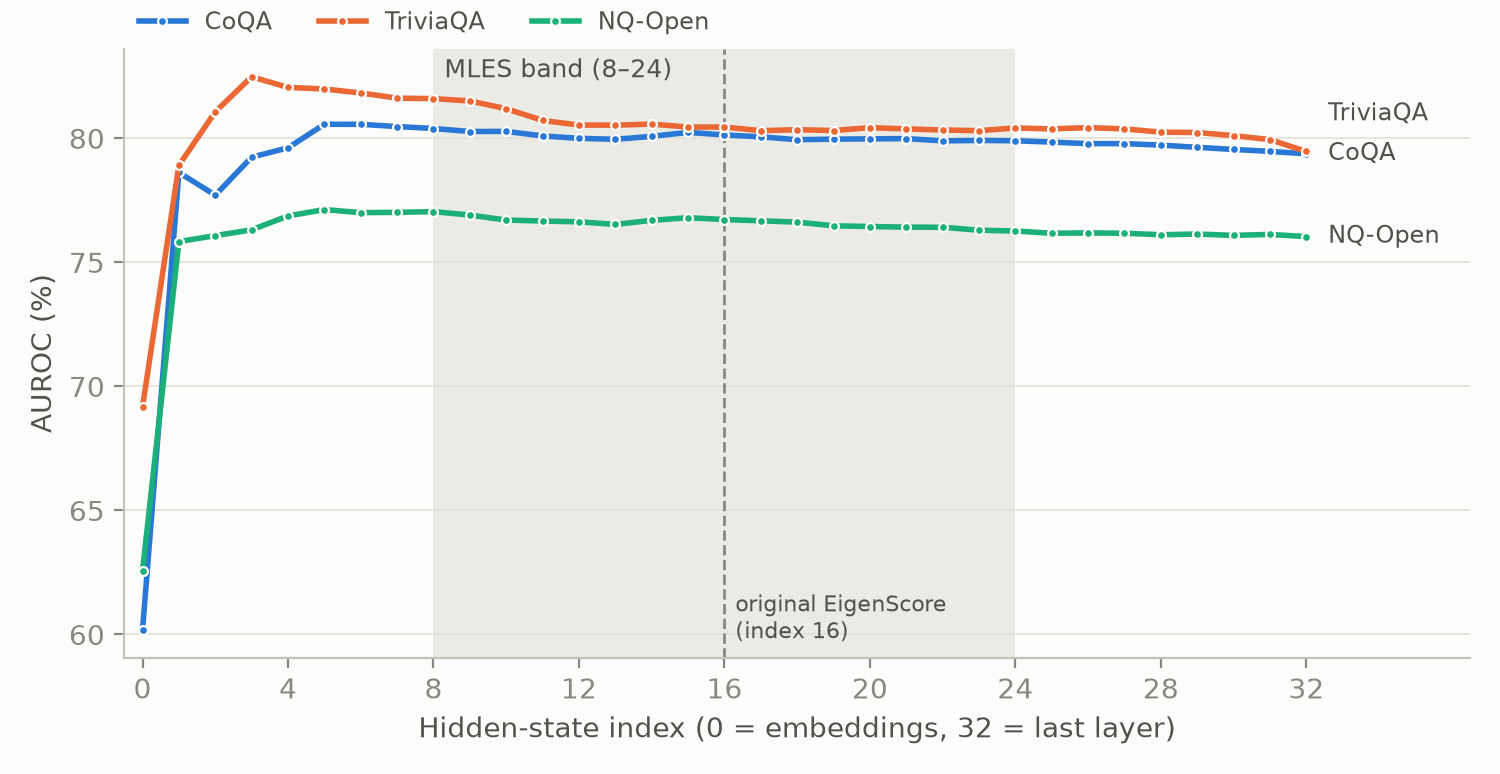
\includegraphics[width=\columnwidth]{figures/per_layer_auroc.png}
\caption{AUROC of single-layer EigenScore at every hidden-state index of Llama-2-7B. The shaded band marks the layers averaged by the multi-layer variant, and the dashed line the middle layer used by EigenScore.}
\label{fig:layers}
\end{figure}

\textbf{Variants of EigenScore that did not help.} Before arriving at the fusion, we evaluated three modifications of the internal signal on all datasets (Table~\ref{tab:negative}). Averaging EigenScore over layers 8--24 changed AUROC by $-0.1$ points on every dataset, consistent with the flat profile in Figure~\ref{fig:layers}. Normalising the embeddings to unit length had no significant effect. A score based on the instability of the sample geometry across layers was clearly inferior. These results indicate that refining the internal signal alone yields little improvement, whereas adding a different kind of evidence does.

\begin{table*}[t]
\centering
\caption{Difference in AUROC (points, 95\% CI) between EigenScore variants and the original EigenScore.}
\label{tab:negative}
\small
\begin{tabular}{@{}lccc@{}}
\toprule
Variant & CoQA & TriviaQA & NQ-Open \\
\midrule
Multi-layer average (layers 8--24) & $-0.1$ [$-0.2$, $0.0$] & $-0.1$ [$-0.4$, $+0.2$] & $-0.1$ [$-0.3$, $+0.1$] \\
Unit-length embeddings (multi-layer) & $+0.1$ [$-1.2$, $+1.5$] & $+0.9$ [$-0.3$, $+2.0$] & $-0.6$ [$-2.0$, $+0.7$] \\
Cross-layer instability & $-3.2$ [$-5.1$, $-1.2$] & $-1.8$ [$-3.2$, $-0.4$] & $-4.3$ [$-6.9$, $-1.9$] \\
\bottomrule
\end{tabular}
\end{table*}

\textbf{Computational cost.} TRI and CTC reuse the samples of EigenScore, so they add no generation cost. Ranking $N$ questions requires $O(N\log N)$ operations, which is negligible compared with sampling. With the 4-bit model, the complete pipeline used at most 5.1~GB of GPU memory.

%=====================================================================
\section{Related Work}\label{sec:related}
\textbf{Uncertainty estimation.} Token-level uncertainty, such as predictive entropy and its length-normalised form, has been widely used to estimate the reliability of generated text~\cite{malinin2021}. Kuhn et al.~\cite{kuhn2023} and Farquhar et al.~\cite{farquhar2024} propose semantic entropy, which clusters sampled answers by meaning before computing the entropy.

\textbf{Self-consistency.} SelfCheckGPT~\cite{manakul2023} and the black-box measures of Lin et al.~\cite{lin2023generating} detect hallucinations from the agreement between sampled answers in the language space, without access to the internal states of the model.

\textbf{Internal states.} INSIDE~\cite{chen2024inside} measures the divergence of sampled answers in the embedding space through EigenScore and proposes test-time feature clipping for overconfident generations. LLM-Check~\cite{sriramanan2024} applies eigenvalue analysis to the hidden states and attention maps of a single response. Massive activations, i.e., a few hidden dimensions with very large values~\cite{sun2024massive}, motivated our normalisation variant.

\textbf{Evaluation.} Janiak et al.~\cite{janiak2025} show that ROUGE-based correctness labels can inflate the AUROC of hallucination detectors and that simple baselines are often competitive. This motivates our comparison with strong lexical baselines and our held-out protocol.

In contrast to these works, the present study combines internal, lexical and token-level evidence without training and from the samples that a sampling-based detector already requires.

%=====================================================================
\section{Conclusion}\label{sec:conclusion}
In this paper, we studied the training-free combination of internal, lexical and token-level evidence for hallucination detection. Experiments with Llama-2-7B on three question-answering benchmarks show that a rank fusion of the three signals improves on EigenScore on every dataset, including the two held-out datasets, without additional generations or labelled data. The analysis indicates that agreement-based and confidence-based signals fail on different questions, in particular on self-consistent hallucinations, whereas refinements of the internal signal alone yield little improvement.

\textbf{Limitations.} The study has the following limitations. First, correctness is determined with ROUGE-L, which may inflate absolute AUROC values~\cite{janiak2025}; paired differences share the same labels and are less affected, but an evaluation with human or LLM-based judgements is still required. Second, a single model with 7B parameters in 4-bit precision is evaluated on 1,000 questions per dataset. Third, the ranks are computed relative to a reference pool, so a strong domain shift between the pool and the deployment questions may distort them. Finally, the internal signal requires access to the hidden states and therefore applies to open-weight models only.

\textbf{Future scope.} In future, the study will be extended to further model families and sizes, to evaluation with LLM-based correctness judgements, and to lightweight learned fusion weights.

\section*{Acknowledgment}
The authors thank Dr.~Venkata Phanikrishna, Indian Institute of Information Technology Vadodara -- International Campus Diu, for guidance throughout this work.

%=====================================================================
\begin{thebibliography}{99}
\bibitem{farquhar2024} S.~Farquhar, J.~Kossen, L.~Kuhn, and Y.~Gal, ``Detecting hallucinations in large language models using semantic entropy,'' \emph{Nature}, vol.~630, pp.~625--630, 2024.
\bibitem{malinin2021} A.~Malinin and M.~Gales, ``Uncertainty estimation in autoregressive structured prediction,'' in \emph{Proc. Int. Conf. Learn. Represent. (ICLR)}, 2021.
\bibitem{lin2023generating} Z.~Lin, S.~Trivedi, and J.~Sun, ``Generating with confidence: Uncertainty quantification for black-box large language models,'' arXiv:2305.19187, 2023.
\bibitem{manakul2023} P.~Manakul, A.~Liusie, and M.~J.~F. Gales, ``SelfCheckGPT: Zero-resource black-box hallucination detection for generative large language models,'' in \emph{Proc. Conf. Empirical Methods Natural Lang. Process. (EMNLP)}, 2023.
\bibitem{kuhn2023} L.~Kuhn, Y.~Gal, and S.~Farquhar, ``Semantic uncertainty: Linguistic invariances for uncertainty estimation in natural language generation,'' in \emph{Proc. Int. Conf. Learn. Represent. (ICLR)}, 2023.
\bibitem{chen2024inside} C.~Chen, K.~Liu, Z.~Chen, Y.~Gu, Y.~Wu, M.~Tao, Z.~Fu, and J.~Ye, ``INSIDE: LLMs' internal states retain the power of hallucination detection,'' in \emph{Proc. Int. Conf. Learn. Represent. (ICLR)}, 2024.
\bibitem{sriramanan2024} G.~Sriramanan, S.~Bharti, V.~S. Sadasivan, S.~Saha, P.~Kattakinda, and S.~Feizi, ``LLM-Check: Investigating detection of hallucinations in large language models,'' in \emph{Adv. Neural Inf. Process. Syst. (NeurIPS)}, 2024.
\bibitem{lin2004rouge} C.-Y. Lin, ``ROUGE: A package for automatic evaluation of summaries,'' in \emph{Text Summarization Branches Out}, 2004, pp.~74--81.
\bibitem{reddy2019coqa} S.~Reddy, D.~Chen, and C.~D. Manning, ``CoQA: A conversational question answering challenge,'' \emph{Trans. Assoc. Comput. Linguist.}, vol.~7, pp.~249--266, 2019.
\bibitem{joshi2017triviaqa} M.~Joshi, E.~Choi, D.~S. Weld, and L.~Zettlemoyer, ``TriviaQA: A large scale distantly supervised challenge dataset for reading comprehension,'' in \emph{Proc. Annu. Meeting Assoc. Comput. Linguist. (ACL)}, 2017.
\bibitem{lee2019latent} K.~Lee, M.-W. Chang, and K.~Toutanova, ``Latent retrieval for weakly supervised open domain question answering,'' in \emph{Proc. Annu. Meeting Assoc. Comput. Linguist. (ACL)}, 2019.
\bibitem{kwiatkowski2019natural} T.~Kwiatkowski \emph{et al.}, ``Natural Questions: A benchmark for question answering research,'' \emph{Trans. Assoc. Comput. Linguist.}, vol.~7, pp.~453--466, 2019.
\bibitem{touvron2023llama} H.~Touvron \emph{et al.}, ``Llama 2: Open foundation and fine-tuned chat models,'' arXiv:2307.09288, 2023.
\bibitem{dettmers2023qlora} T.~Dettmers, A.~Pagnoni, A.~Holtzman, and L.~Zettlemoyer, ``QLoRA: Efficient finetuning of quantized LLMs,'' in \emph{Adv. Neural Inf. Process. Syst. (NeurIPS)}, 2023.
\bibitem{holm1979} S.~Holm, ``A simple sequentially rejective multiple test procedure,'' \emph{Scand. J. Statist.}, vol.~6, no.~2, pp.~65--70, 1979.
\bibitem{sun2024massive} M.~Sun, X.~Chen, J.~Z. Kolter, and Z.~Liu, ``Massive activations in large language models,'' in \emph{Proc. Conf. Lang. Model. (COLM)}, 2024.
\bibitem{janiak2025} D.~Janiak, J.~Binkowski, A.~Sawczyn, B.~Gabrys, R.~Shwartz-Ziv, and T.~Kajdanowicz, ``The illusion of progress: Re-evaluating hallucination detection in LLMs,'' arXiv:2508.08285, 2025.
\end{thebibliography}

\end{document}
